\documentclass[12pt,a4paper]{article}
\usepackage{graphicx}
\usepackage{csquotes}
\usepackage{centernot}
\usepackage{mathtools}
\usepackage{amsfonts}
\usepackage{algorithm}
\usepackage{amsthm}
\usepackage{caption}
\usepackage{array}
\usepackage{dsfont}
\usepackage{ amssymb }
\usepackage{blindtext}
\usepackage{hyperref}
\usepackage{amsmath}
\usepackage{breqn}
\usepackage{tikz}
\usepackage{pgfplots}
\renewcommand{\arraystretch}{1.3}
\usepackage[a4paper]{geometry}
\usepackage{multirow}
\usepackage{graphicx}
\usepackage[all]{xy}
\newtheorem{theorem}{Theorem}
\theoremstyle{definition}
\newtheorem{definition}{Definition}[section]
\theoremstyle{remark}
\newtheorem*{remark}{Remark}
\usepackage[noend]{algpseudocode}
\pgfmathdeclarefunction{poiss}{1}{%
	\pgfmathparse{(#1^x)*exp(-#1)/(x!)}%
}

\algrenewcommand\algorithmicrequire{\textbf{Input:}}
\newcommand\ddfrac[2]{\frac{\displaystyle #1}{\displaystyle #2}}
\newcommand\at[2]{\left.#1\right|_{#2}}
\usepackage{mathtools}
\DeclarePairedDelimiter{\ceil}{\lceil}{\rceil}
\graphicspath{ {images} }
%opening
\title{Bayesian Regression with COVID-19 spread data}
\author{Michele Guerrini, Davide Mozzi, Carlos Santillán}
\begin{document}
	\maketitle
	\begin{abstract}
		We present a Bayesian regression model for predicting the number of patients in a hospital and the ICU with COVID -19, given the number of patients in the same hospital and ICU, the number of new positive subjects and the region color of the previous week. 
	\end{abstract}
	
	\tableofcontents
	\newpage
	\section{Problem Description and Dataset}
	\subsection{Problem description}
	We are given the problem of predicting the number of patients in a hospital and the ICU 7 days from the current date. The prediction is based on the current date's patients both in the hospital and the ICU, new positive subjects, the average number of new positive subjects over the previous 7 days, and the color of the region. We tackle the problem via Bayesian regression
	\subsection{Dataset description}
	The dataset contains 205 entries. Each entry corresponds to a date with the following features
	\begin{enumerate}
		\item \textbf{newpos:} Number of newly detected COVID-19 positive subjects. An integer value.
		\item \textbf{intcar:} 	Number of COVID patients in the ICU. An integer value.
		\item \textbf{hosp:} Number of COVID patients at the hospital. An integer value.
		\item \textbf{newpos\_av7D:} Average number of newly detected COVID-19 positive subjects over the previous 7 days. A float value.
		\item \textbf{color:} Color of the region over the previous 7 days. String that can contain the following values: \textit{Bianca}, \textit{Gialla}, \textit{Arancione}, \textit{Rossa}.
		\item \textbf{day:} Current date. String in R date format.
		\item \textbf{hospH8:} A target variable, the number of COVID patients at the hospital 7 days from now.
		\item \textbf{intcarH8:} A target variable, the number of COVID patients in the ICU 7 days from now.
		\item \textbf{dayH8:} The current date plus 7 days. 
	\end{enumerate}
	We will extend this by adding a categorical variable \textbf{season}, which will have values: \textit{winter}, \textit{spring}, \textit{summer}, \textit{fall}.
	\subsection{Data exploration}
	We start by looking at a pairs plot of the \textbf{newpos}, \textbf{intcar}, \textbf{hosp}, \textbf{newpos-avg7D}, and \textbf{hospH8}. The pairs plot contains a kernel density estimation of the distribution along the diagonal, the estimations are distinguished by color of the region. We also see the scatter plots for each pair of features, and the correlations between them for each region.
	\begin{figure}[htb!]
		\centering
		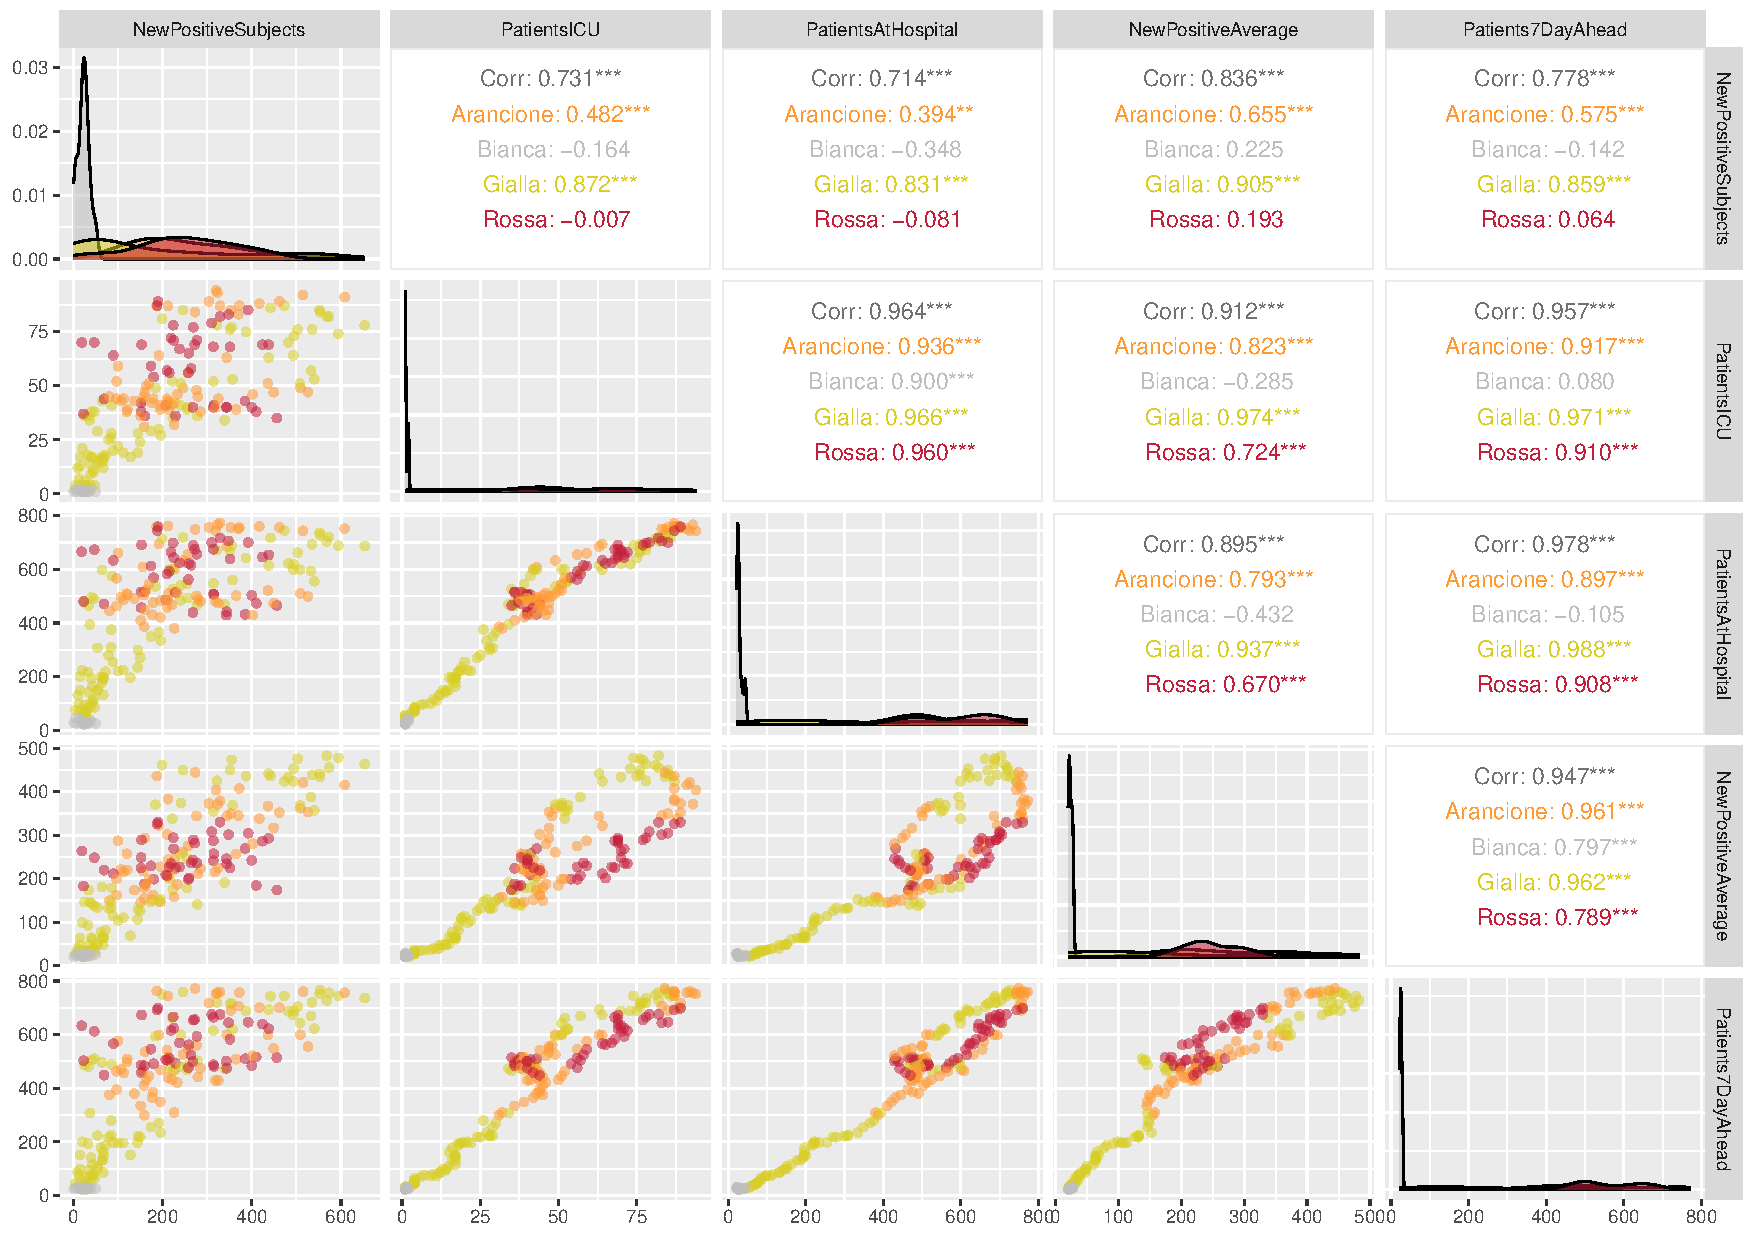
\includegraphics[width=150mm, height=115mm,scale=0.5]{corrplot.pdf}
			\caption{Pairs plot between the features and the number of patients at the hospital 7 days from now}
	\end{figure}
	
	
	We can immediately see an almost linear relationship between the number of patients in the ICU and those at the hospital, suggesting that we may remove one of them. The density plots are as we would expect, the white regions (lower COVID-19 presence) have all the mass concentrated around low values of the features, while the other regions are more spread out and have a center of mass further to the right (higher values). We also see that the relationship between the number of patients at the hospital, and that of 7 days in the future could be linear.
	
	\newpage
	We now look at the correlations with the number of patients in the ICU
		\begin{figure}[htb!]
		\centering
		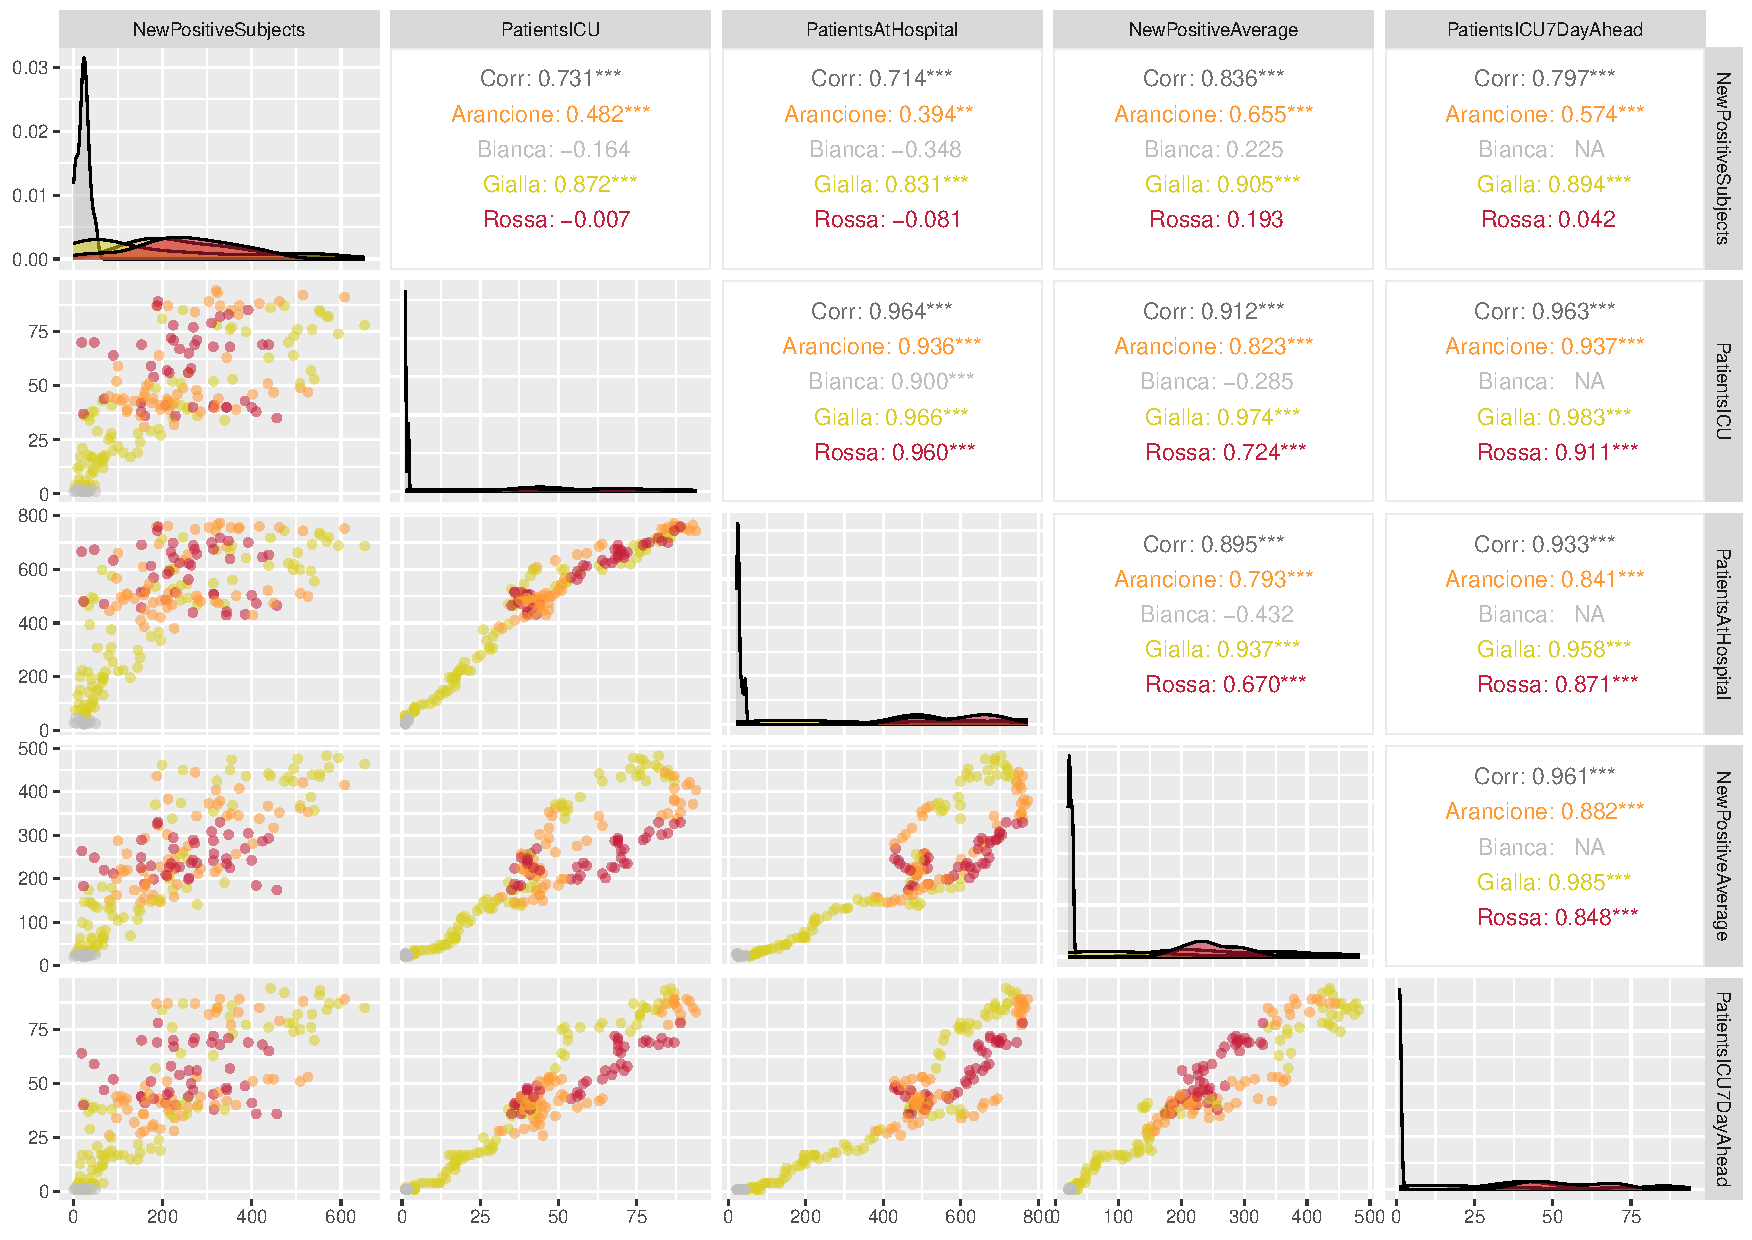
\includegraphics[width=150mm, height=115mm,scale=0.5]{corrplot1.pdf}
		\caption{Pairs plot between the features and the number of patients in the ICU 7 days from now}
	\end{figure}
	
	
	Again, for some of the features the relationship appears to be linear w.r.t. the target variable. Note that where the correlation is marked NA the value is zero. We used the Pearson correlation coefficient $r_{X,Y}$, defined as
	\begin{align*}
		r_{X,Y} = \frac{\sum(x_i-\overline{x})(y_i-\overline{y})}{\sqrt{\sum(x_i-\overline{x})^2\sum(y_i-\overline{y})^2}}
	\end{align*}


    Now we qualitatively assess how much each feature varies via boxplots (Figure 3). A boxplot allows us to see the spread of our data, the boxes themselves contain the interquantile range, the whiskers show the range of the rest of the data. We also mean center the features.
    	\begin{figure}[htb!]
    	\centering
    	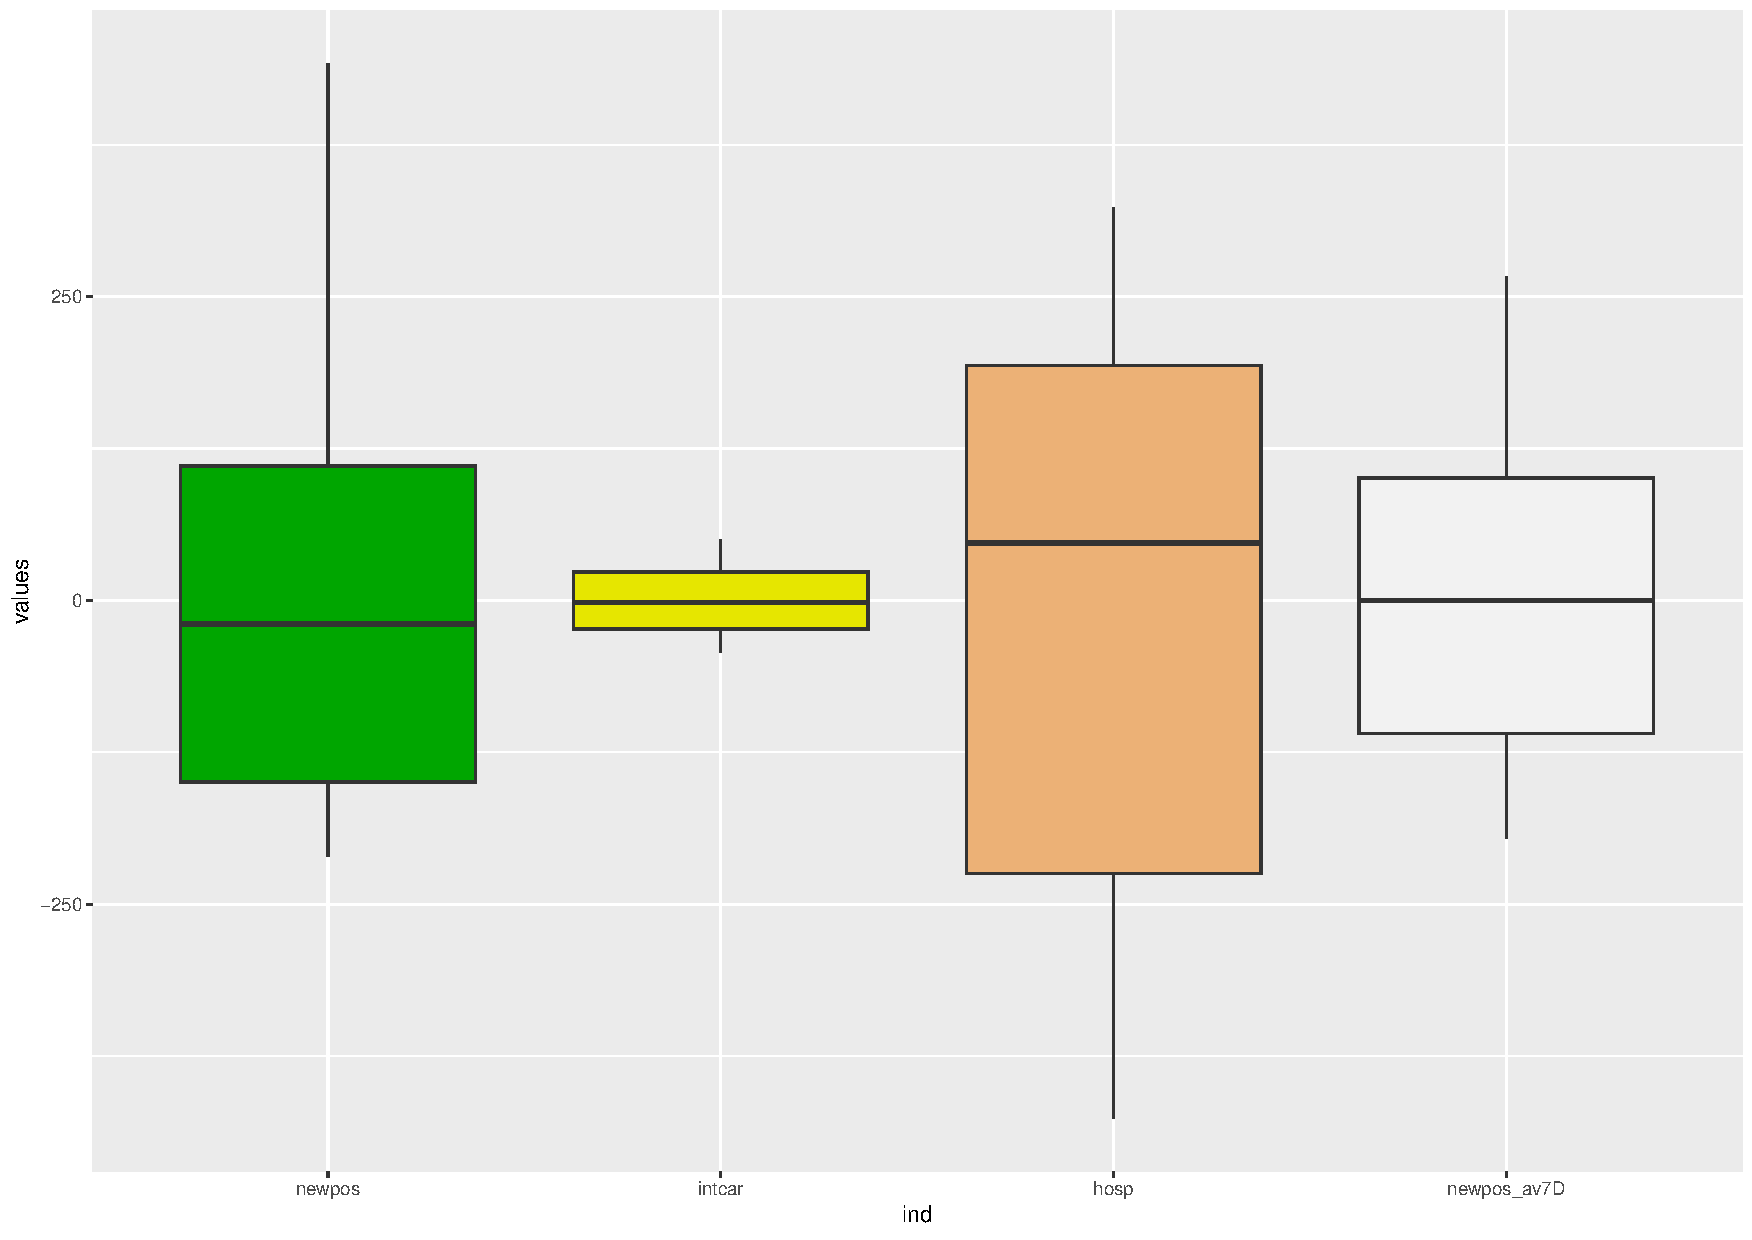
\includegraphics[width=100mm, height=80mm,scale=0.5]{box.pdf}
    	\caption{Boxplot of the mean-centered features}
    \end{figure}
    
    Since the some features vary greatly w.r.t. to others, see \textbf{intcar} and \textbf{hosp}, it could be a conventient to normalize the features. 

Lastly, we take at the correlation matrices of the features. Figure 4 shows the full correlation matrix, no distinction made between regions. 

Figure 5 shows the correlation matrix for each region.
    
\begin{figure}[htb!]
	\centering
	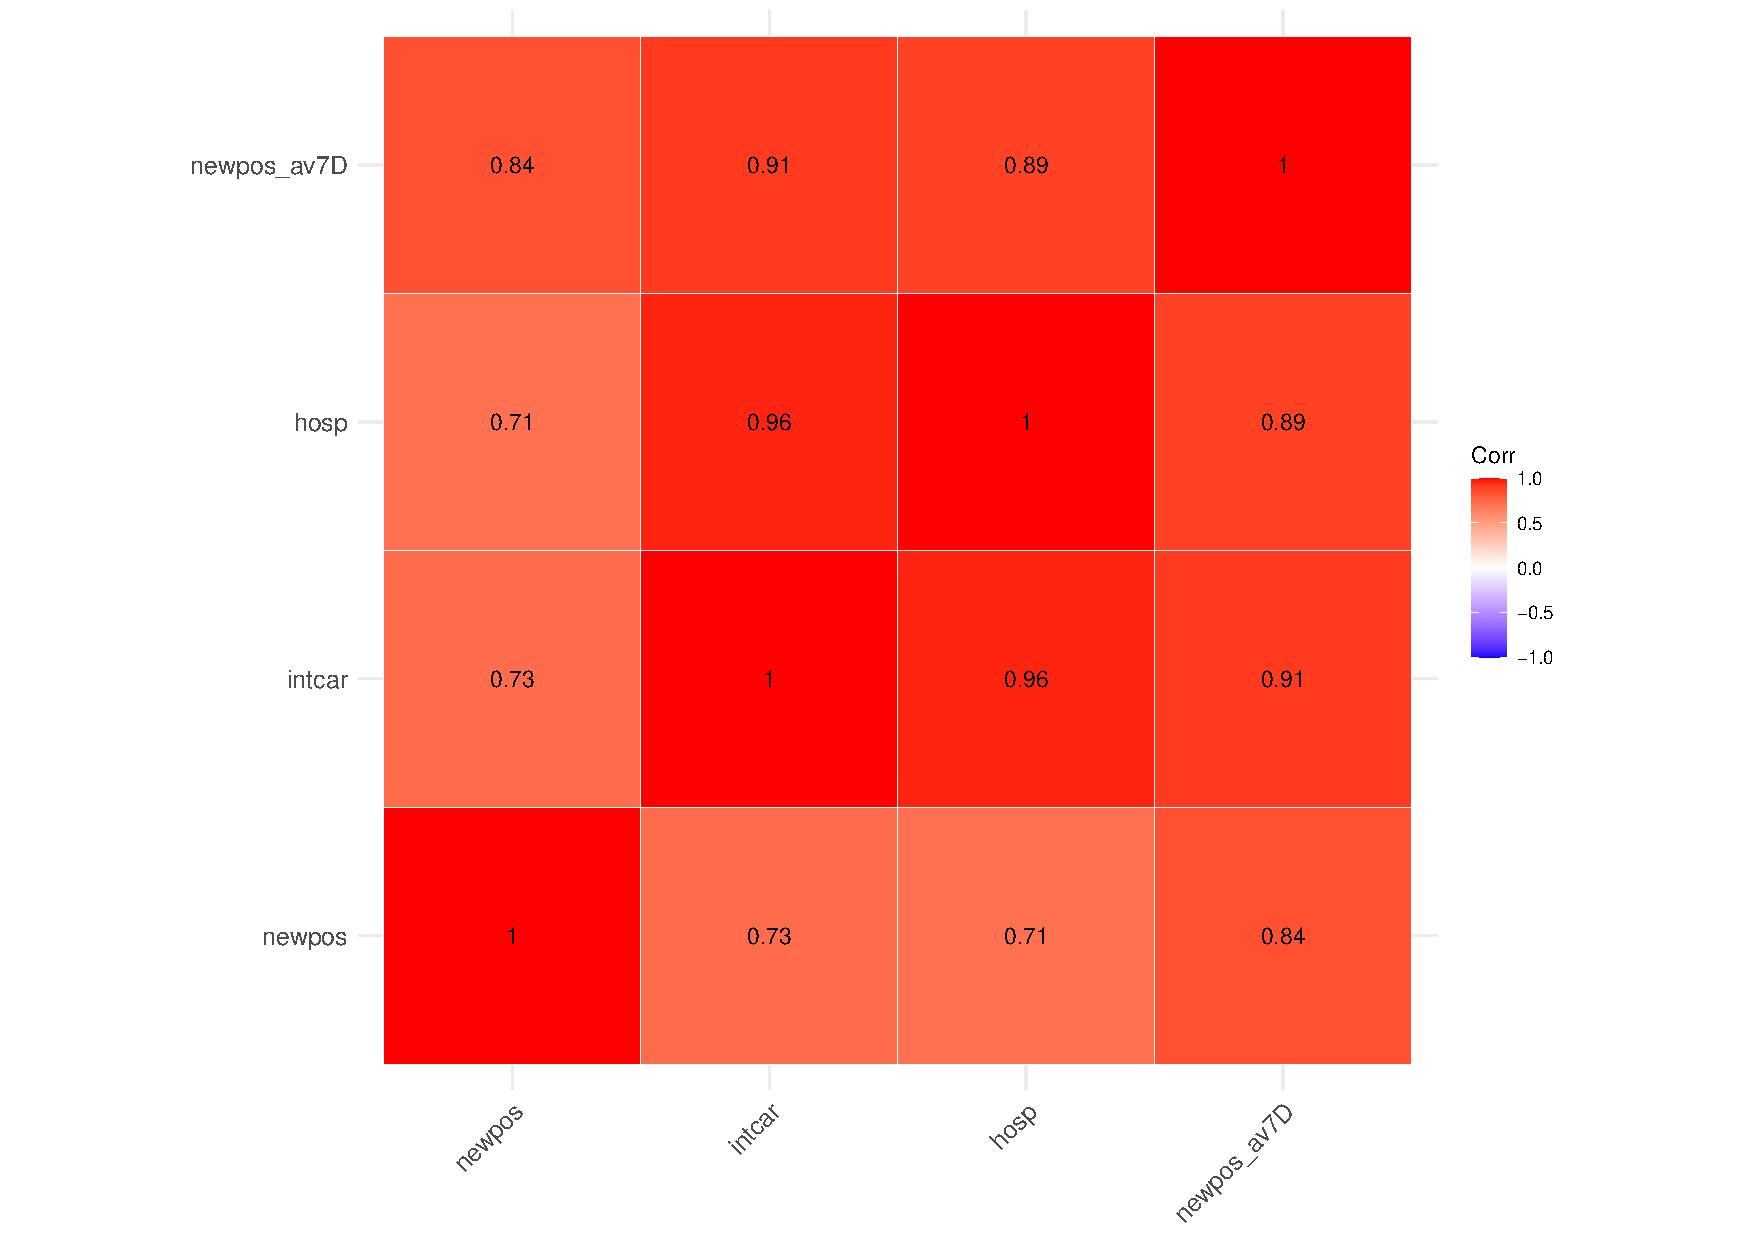
\includegraphics[width=75mm, height=60mm,scale=0.5]{corrmatrix.pdf}
	\caption{Correlation matrix of the features}
\end{figure}
\begin{figure}[htb!]
	\centering
	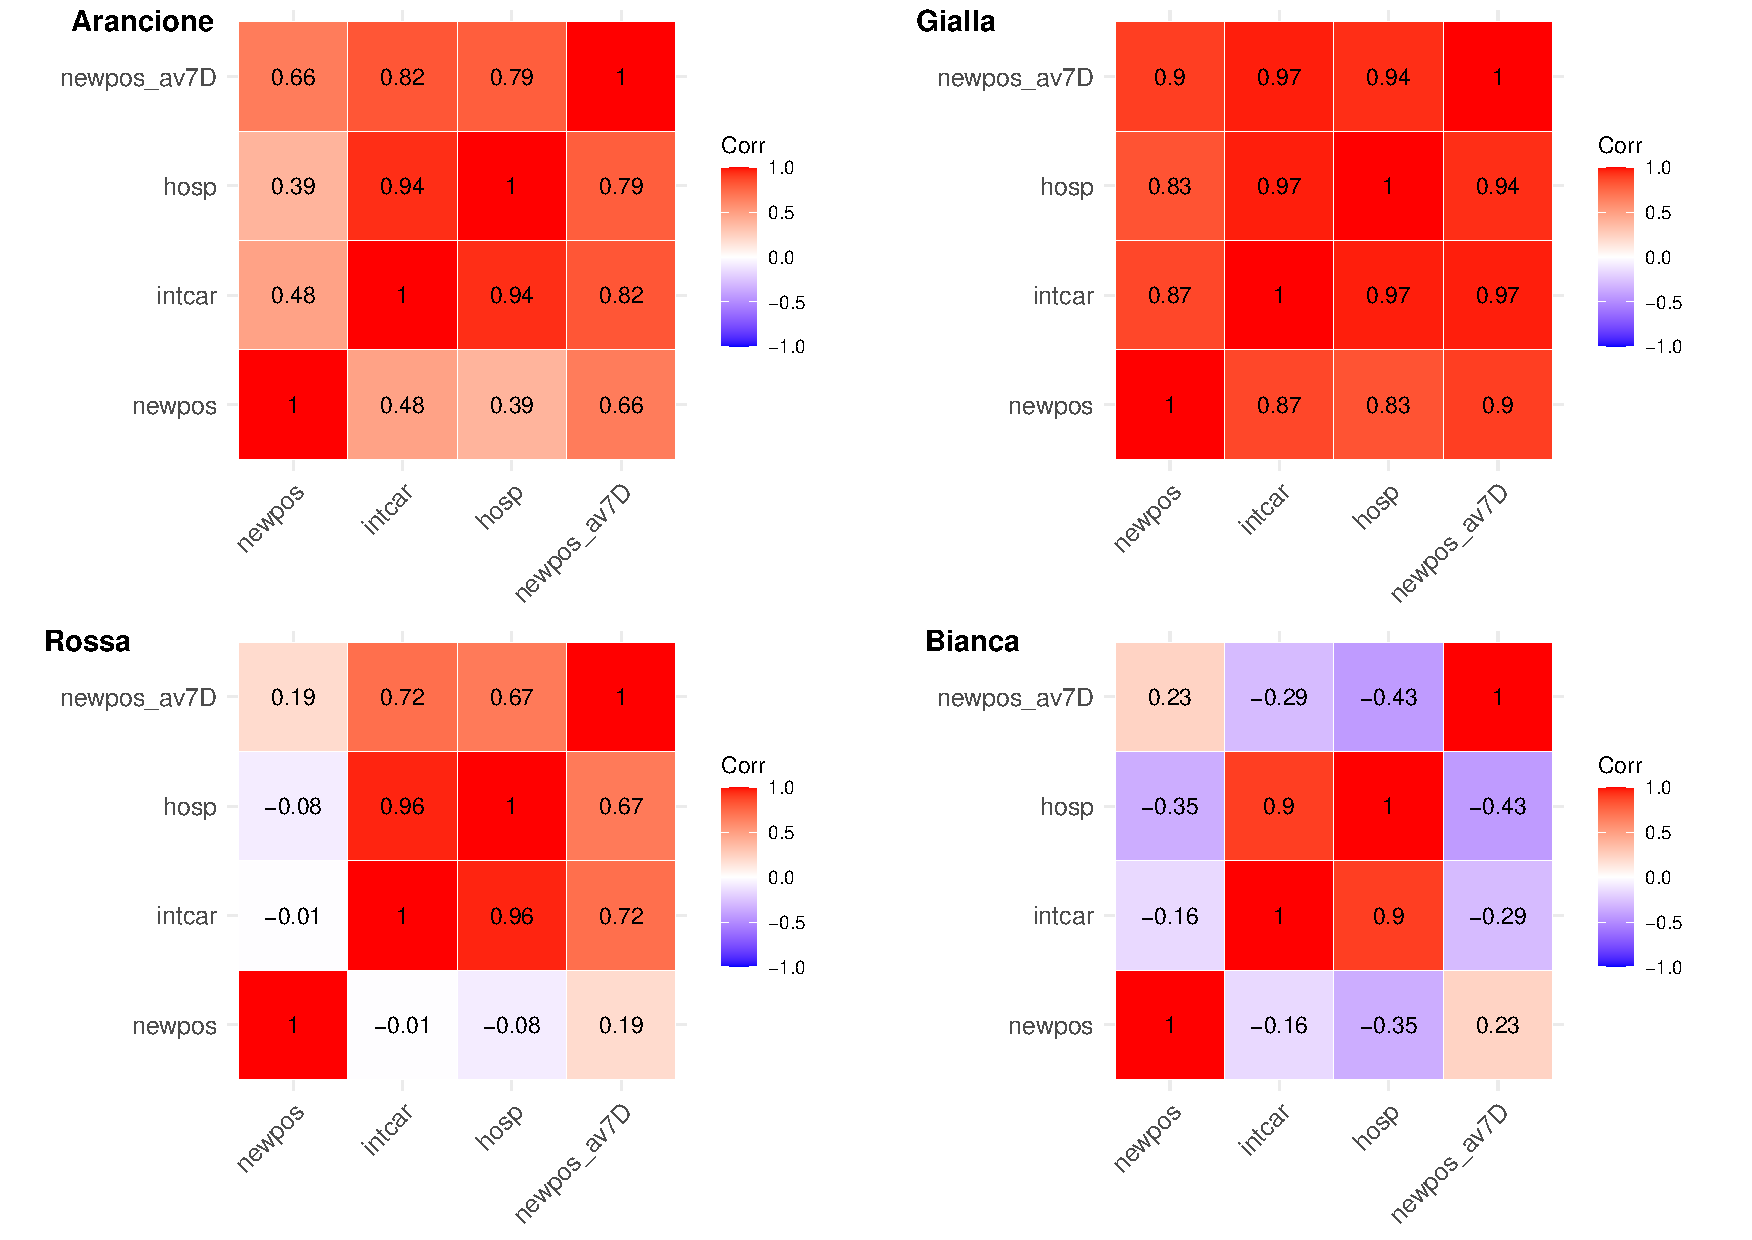
\includegraphics[width=130mm, height=100mm,scale=0.5]{corrmat2.pdf}
	\caption{Correlation matrix of the features per region}
\end{figure}


Before proceeding, we shuffle and split the dataset in training and test sets with a 87/13 ratio. We also normalize the covariates in the training set, but not the target variables.

\clearpage




\section{Model specification}
\subsection{Likelihood and prior}
In the Bayesian setting, we use a Gaussian likelihood 
\begin{align*}
	y|\beta,\sigma^2,X \sim \mathcal{N}_n(X\beta,\sigma^2I_n)
\end{align*}

For the prior we initially used default one provided by BAS. BAS uses an approximation of the Zellner-Siow prior 

	\begin{align*}
	\beta = (\beta_1, \dots, \beta_k)|\sigma^2, \alpha, X &\sim \mathcal{N}_k(0, \alpha\sigma^2(X^TX)^{-1}) \\
	\sigma^2|X,\alpha &\sim \pi(\sigma^2) = \sigma^{-2} \\
	1/\alpha &\sim \pi_0 = \Gamma(1/2, n/2)
\end{align*}
BAS sets the hyperparameter $\alpha$ to 1. 

We try to predict each target separately and start with \textbf{hostH8}, we consider a model with all the covariates. In particular, \textbf{color} is considered a categorical variable, which was transformed into 3 binary covariates via one-hot encoding. The model is
\begin{dmath*}
	\textbf{hospH8} = \beta_0 + \beta_1\textbf{gialla} + \beta_2\textbf{arancione} + \beta_3\textbf{rossa} + \beta_4\textbf{newpos} + \beta_5\textbf{intcar} + \beta_6\textbf{hosp} +  \varepsilon
\end{dmath*}

Since we are only using one model which always includes these covariates the probability of them belonging to the model is always 1.  Table 1 shows the posterior means and standard deviations of the coefficients\footnote{Do not confuse them with the actual covariates, these refer to the coefficents $\beta_i$ of $i$-th covariate}


\begin{table}[htb!]
	\centering
	\begin{tabular}{|c|c|c|}
		\hline
		Coefficient          & Posterior mean & Posterior standard deviation \\ \hline
		Intercept          & -0.004298      & 0.012938                     \\ \hline
		\textbf{gialla}    & -0.092490      & 0.058380                     \\ \hline
		\textbf{arancione} & -0.166263      & 0.070069                     \\ \hline
		\textbf{rossa}     & -0.134449      & 0.072101                     \\ \hline
		\textbf{newpos}    & 0.147965       & 0.019453                     \\ \hline
		\textbf{intcar}    & 0.057368       & 0.053409                     \\ \hline
		\textbf{hosp}      & 0.841135       & 0.057545                     \\ \hline
	\end{tabular}
	\caption{Posterior means and standard deviations of the first model}
\end{table}
\begin{figure}[htb!]
	\centering
	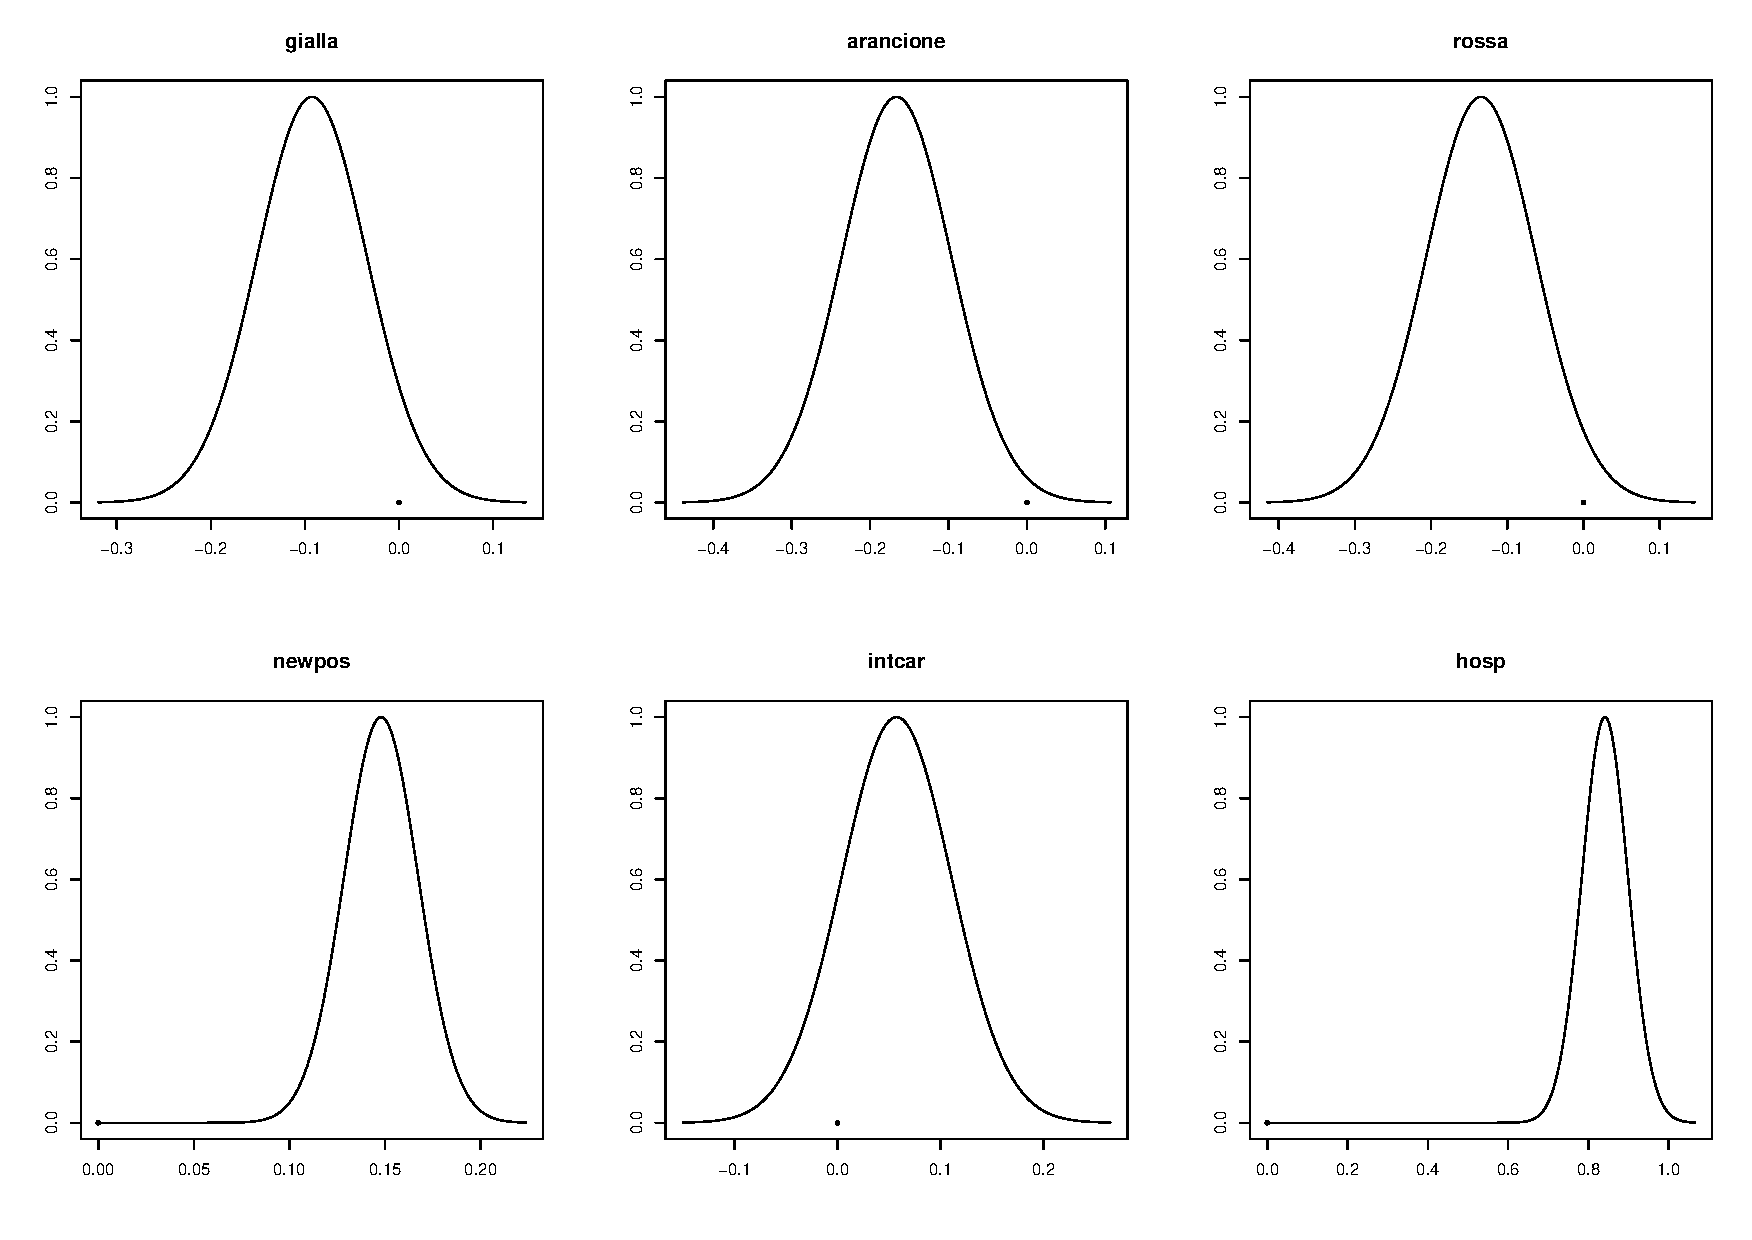
\includegraphics[width=140mm, height=100mm,scale=0.5]{posterior_first_model.pdf}
	\caption{Posterior distributions of each coefficient}
\end{figure}


Figure 6 shows the posterior distributions of the coefficients.


We perform inference on the test set, for which BAS uses the posterior predictive distribution. We recall that in general the predictive posterior distribution is computed as 
	\begin{align*}
	\int \pi(y_{\text{new}}|\sigma^2,\beta,X_{\text{new}})\pi(\sigma^2,\beta|y,X)\,d\sigma^2d\beta
\end{align*}

We use the mean square error MSE
\begin{align*}
	\text{MSE} = \frac{1}{n}\sum_{i=1}^{n}(y_i-\hat{y_i})^2
\end{align*}
where $y_i$ is the actual number of people hospitalized after 7 days, and $\hat{y_i}$ is our prediction. We obtain a MSE of 0.02659245.

For the target variable \textbf{intcarH8} we consider an almost identical model

\begin{dmath*}
	\textbf{intcarH8} = \beta_0 + \beta_1\textbf{gialla} + \beta_2\textbf{arancione} + \beta_3\textbf{rossa} + \beta_4\textbf{newpos} + \beta_5\textbf{intcar} + \beta_6\textbf{hosp} + \varepsilon
\end{dmath*}

The MSE is 0.07319181. We show a more in-depth posterior analysis with the final model. Please note that the covariates in the test set are normalized with the training set's mean and standard deviation.

Another model we tried was one that considered the \textbf{color} feature as an ordinal variable, note that we used the same prior.  The covariate starts from 1 (\textit{Bianca}) and ends in 4 (\textit{Rossa}). For \textbf{intcarH8} the model becomes
\begin{dmath*}
	\textbf{intcarH8} = \beta_0 + \beta_1\textbf{color}  + \beta_2\textbf{newpos} + \beta_3\textbf{intcar} \\+ \beta_4\textbf{hosp}  + \varepsilon
\end{dmath*}
which yields a MSE of 0.07816081, slightly worse than the error for the previous model. The same goes for \textbf{hospH8}, this is consistent across multiple shufflings and retrainings of the model, so we decide to drop this variant of our model. 

We change prior to Zellner's g-prior, of the form
	\begin{align*}
	\beta = (\beta_1,\dots, \beta_k)|\sigma^2 &\sim \mathcal{N}_k(0, \alpha\sigma^2(X^TX)^{-1}) \\
	(\beta_0, \sigma^2) &\sim \pi(\beta_0, \sigma^2) = \sigma^{-2}
\end{align*}
However, we start by setting $\alpha$ to infinity, so the data completely determines our model. We also add the covariate \textbf{newpos\_av7D}, and also perform model selection and set a uniform prior on all possible models that use a subset of these covariates.

We obtain the following posterior probabilities for each covariate
\begin{table}[htb!]
	\centering
	\begin{tabular}{|c|c|}
		\hline
		Coefficient          & Posterior \\ \hline
		Intercept          & 1.0000000                   \\ \hline
		\textbf{gialla}    & 0.1777365                  \\ \hline
		\textbf{arancione} & 0.1728493                   \\ \hline
		\textbf{rossa}     & 0.9542922                     \\ \hline
		\textbf{newpos}    & 0.1653874                  \\ \hline
		\textbf{intcar}    & 0.3617246                \\ \hline
		\textbf{hosp}      & 1.0000000        \\ \hline
			\textbf{newpos\_av7D}      & 1.0000000        \\ \hline
	\end{tabular}
	\caption{Probabilities of each covariate in the second model}
\end{table}


As we can see we certainly want to include the covariates \textbf{rossa}, \textbf{hosp}, and \textbf{newpos\_av7D} in our model. 

Using the same basis for our model, we obtain the following probabilities for the target variable \textbf{intcarH8}
\begin{table}[htb!]
	\centering
	\begin{tabular}{|c|c|}
		\hline
		Coefficient          & Posterior \\ \hline
		Intercept          & 1.0000000                   \\ \hline
		\textbf{gialla}    &0.1136039                 \\ \hline
		\textbf{arancione} & 0.9989177               \\ \hline
		\textbf{rossa}     &0.0934188                 \\ \hline
		\textbf{newpos}    &  0.1316067             \\ \hline
		\textbf{intcar}    & 1.0000000            \\ \hline
		\textbf{hosp}      &0.1067579       \\ \hline
		\textbf{newpos\_av7D}      & 1.0000000        \\ \hline
	\end{tabular}
	\caption{Probabilities of each covariate in the second model for \textbf{intcarH8}}
\end{table}

We observe that the most ``useful" covariates instead are \textbf{arancione}, \textbf{intcar}, and \textbf{newpos\_av7D}.

\subsection{Model selection}

In the case of \textbf{hospH8} the top 5 models have the following posterior probabilities

\begin{table}[htb!]
	\centering
	\begin{tabular}{|c|c|c|c|c|c|}
		\hline
		Models                & Model 1 & Model 2   & Model 3    & Model 4   & Model 5    \\ \hline
		Posterior probability & 0.3755  & 0.2975000 & 0.05410000 & 0.0429000 & 0.04250000 \\ \hline
	\end{tabular}
	\caption{Posterior probabilities of the best 5 models for \textbf{hospH8}}
\end{table}
Figure 7 shows a heatmap-like plot of the posterior probabilities and the inclusion of covariates of each model.

\begin{figure}[htb!]
	\centering
	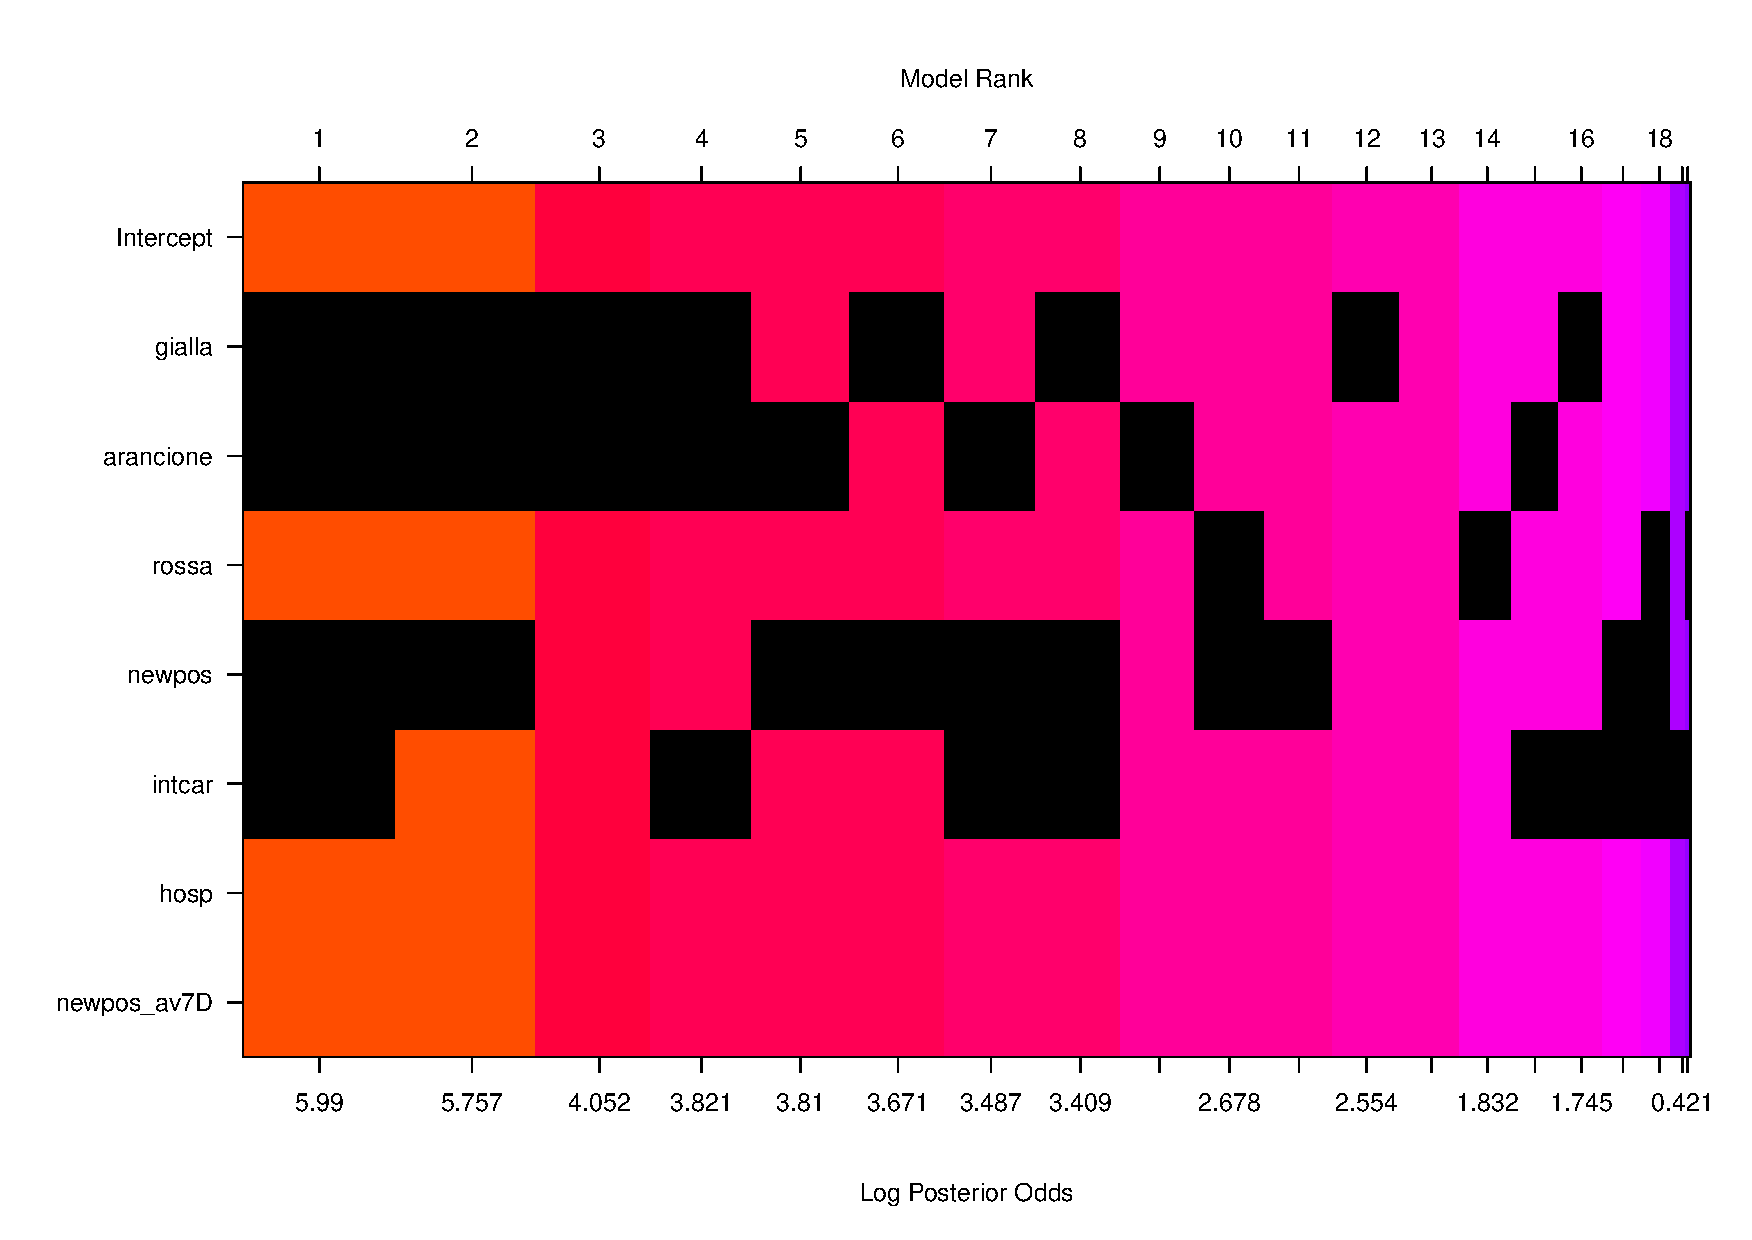
\includegraphics[width=100mm, height=60mm,scale=0.5]{modelranking.pdf}
	\caption{Model ranking and posterior probabilities }
\end{figure}



Since none of the models have a posterior probability above 50\%, we do not choose the best model, which in this case is model 1, but we use Bayesian model averaging (BMA), the posterior probability of a quantity of interest $\Delta$, computer via BMA, is
\begin{align*}
	\pi(\Delta|\mathbf{y}) = \sum_{j=1}^{2^p}\pi(\Delta| M_j, \mathbf{y})\pi(M_j|\mathbf{y})
\end{align*}
where $p$ is the number of covariates

We then compute our predictions as a weighted average of each model's prediction, where the weights are the model's posterior probabilities
\begin{align*}
	\hat{Y} = \sum_{j=1}^{2^p}\hat{Y}^*_jp(M_j|X)
\end{align*}
The MSE for this aggregate model is 0.01251516, sligthly better than the first model with all the covariates.

The ranking for the models predicting \textbf{intcarH8} is shown in Figure 8
\begin{figure}[htb!]
	\centering
	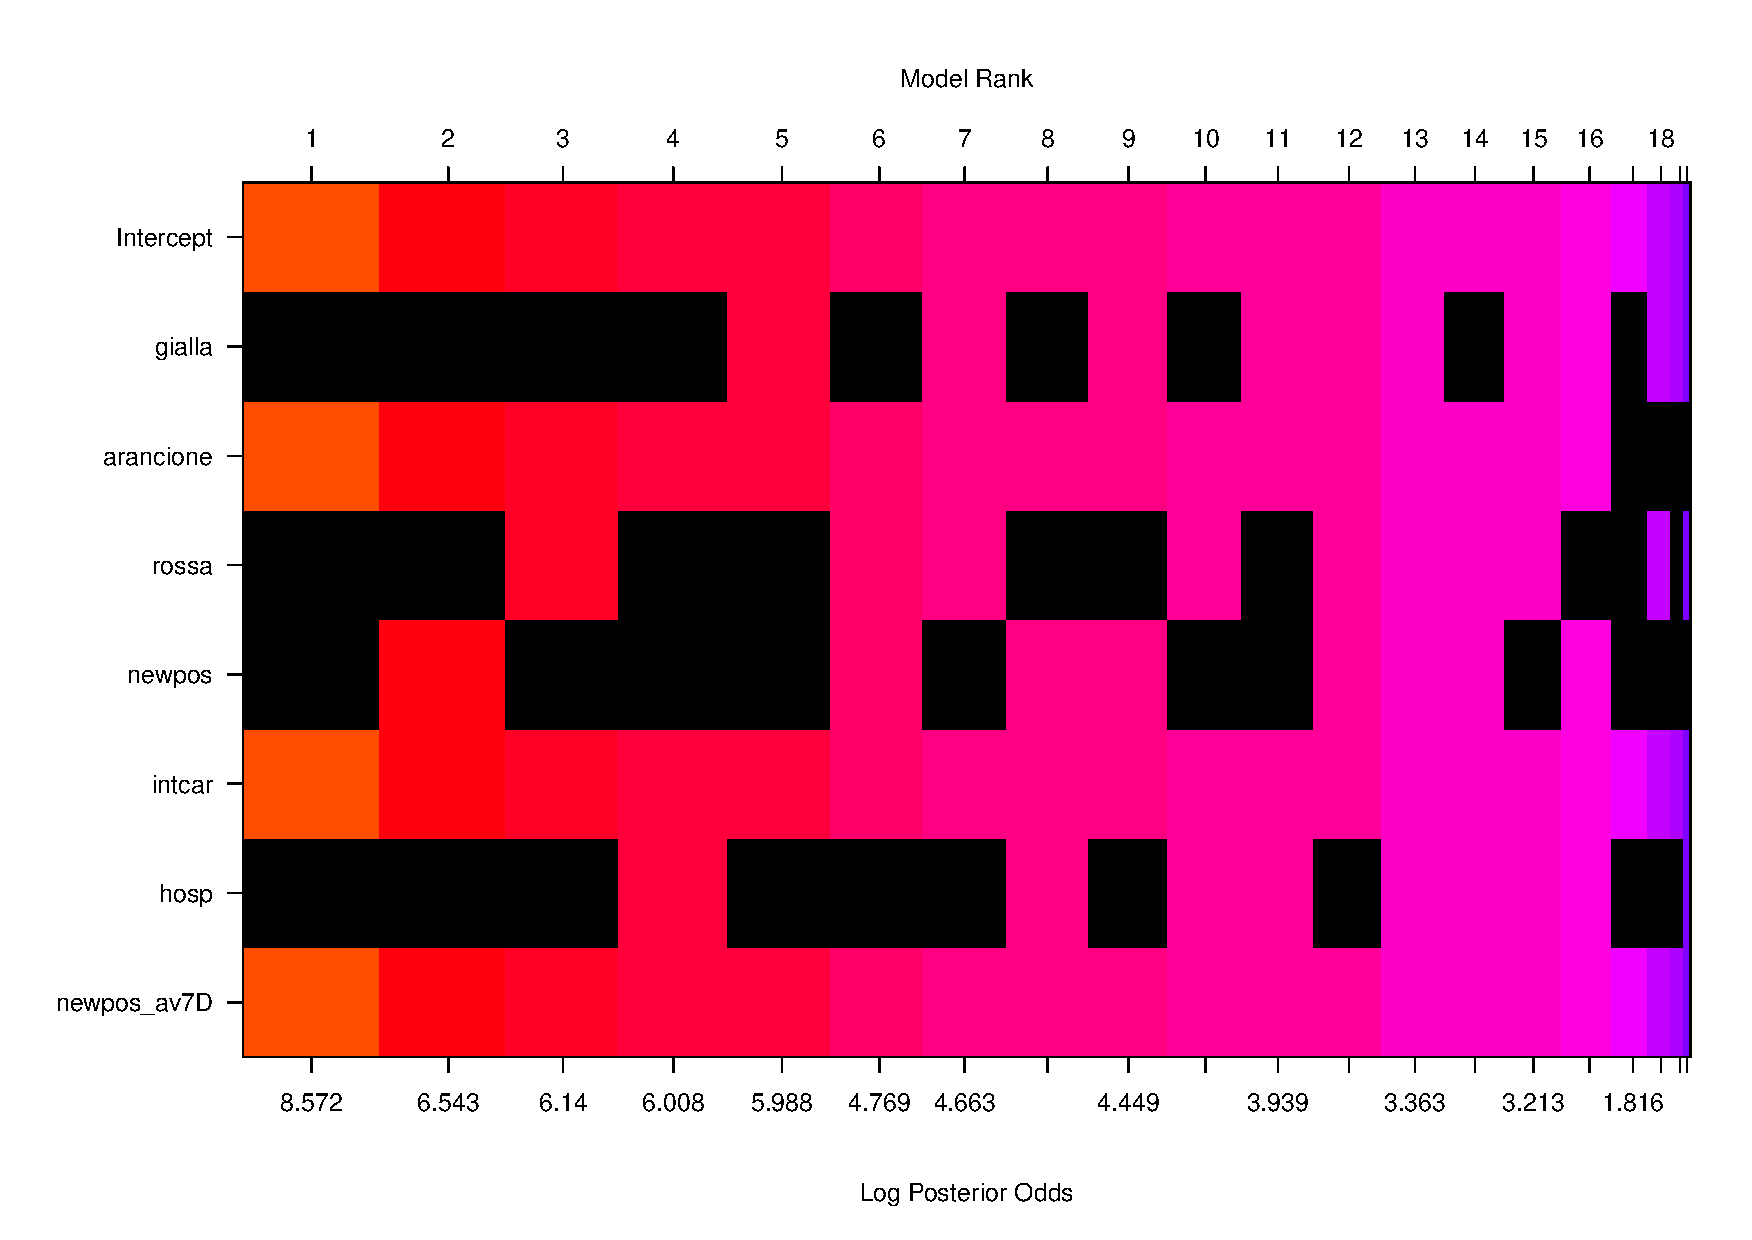
\includegraphics[width=100mm, height=60mm,scale=0.5]{ranking2.pdf}
	\caption{Model ranking for \textbf{intcarH8} }
\end{figure}
For \textbf{intcarH8} the best model has a posterior probability of 65\%, so we could try to use only that one to perform inference. So we choose the model
\begin{dmath*}
	\textbf{intcarH8} = \beta_0 + \beta_1\textbf{arancione} +  \beta_2\textbf{intcar} + \beta_3\textbf{newpos\_av7D} + \varepsilon
\end{dmath*}
which yields a MSE of 0.04632954\footnote{Note that we judge the improve in terms of the MSE over a large number of shufflings and iterations}, better than the one using all the covariates.

We also added a categorical covariate \textbf{season}, as mentioned in the first section. However, it yielded similar slightly worse results in terms of MSE (for \textbf{intcarH8} 0.0495), so we decided to drop it. 
\newpage
\section{Posterior analysis}
\subsection{Posterior distributions }
We start with the aggregate model chosen for \textbf{hospH8}. The posterior distributions of the coefficients are
\begin{figure}[htb!]
	\centering
	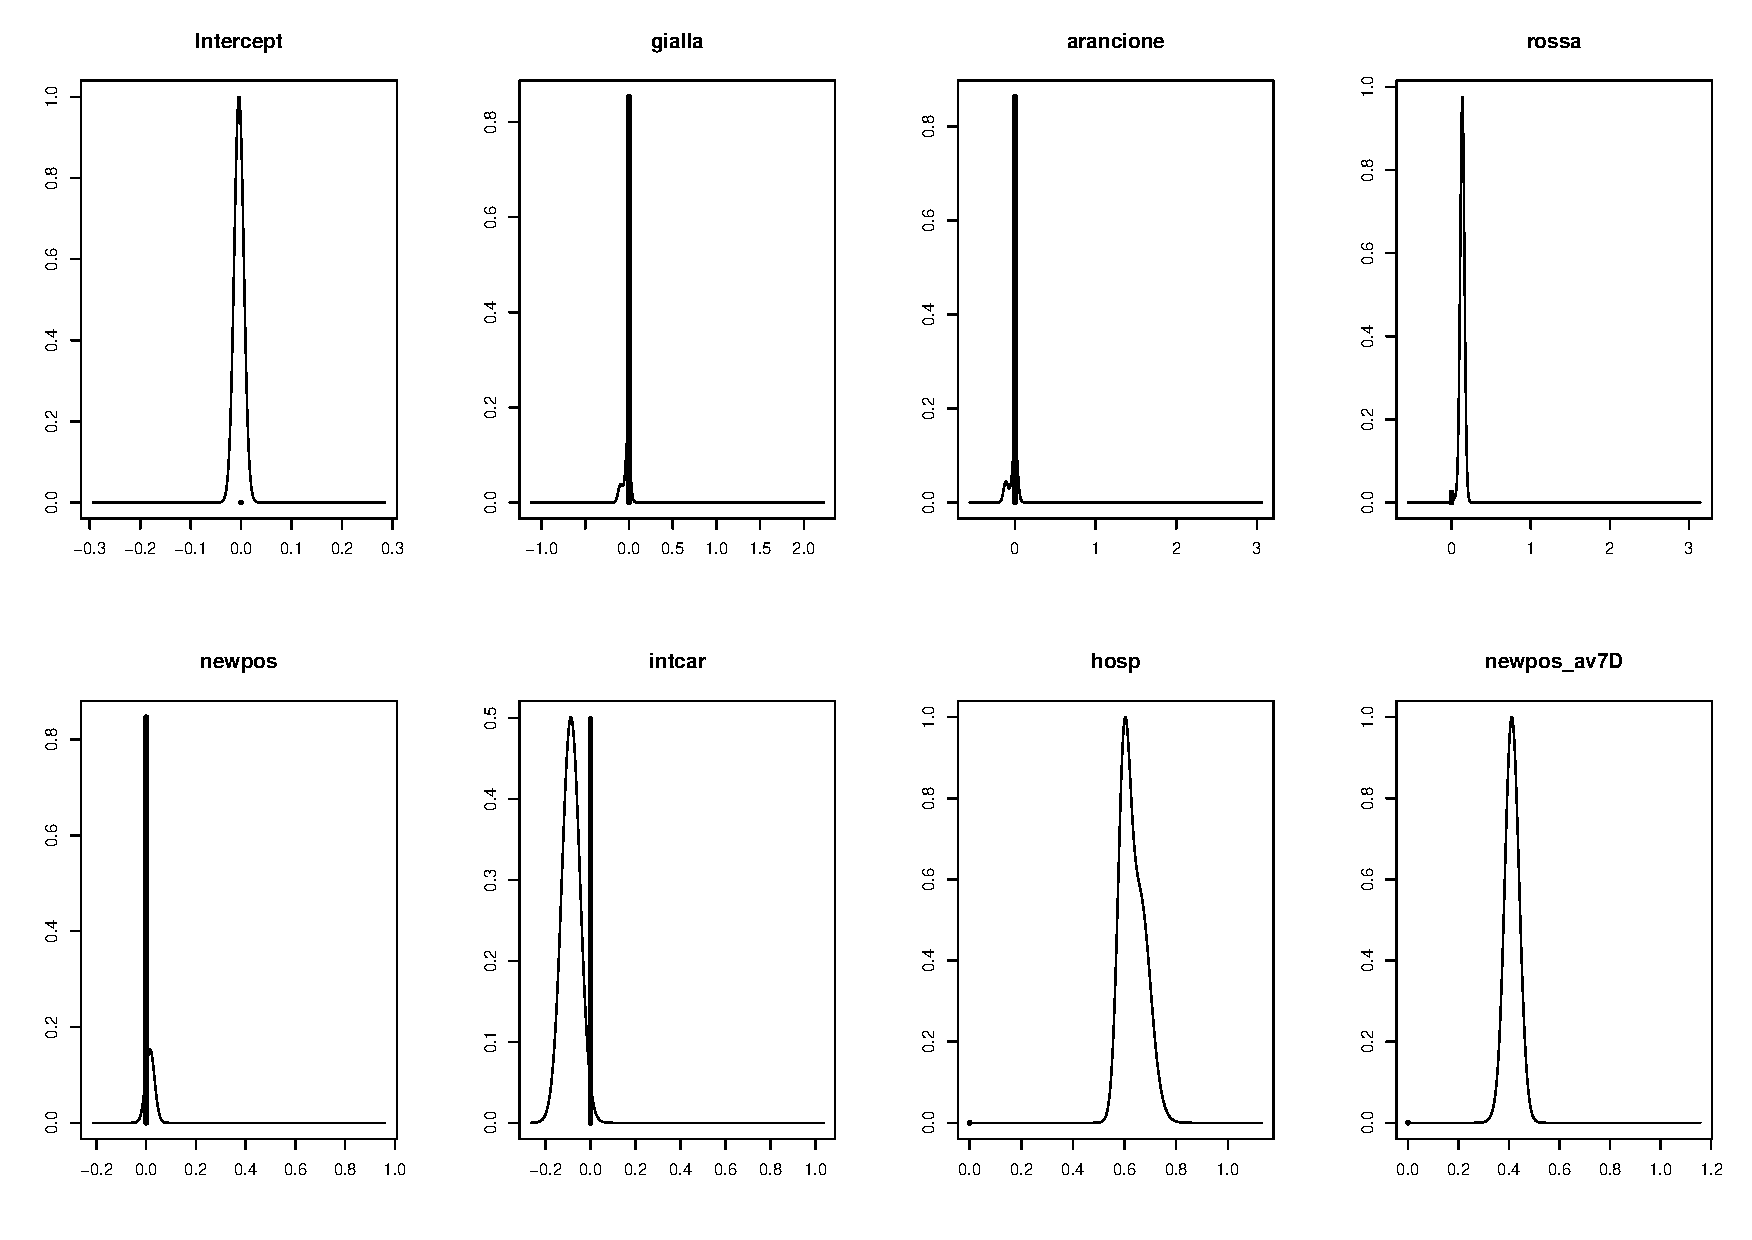
\includegraphics[width=155mm, height=90mm,scale=0.5]{posteriors_1.pdf}
	\caption{Posterior distributions of coefficients for best \textbf{hospH8} model}
\end{figure}

Judging by where they are centered we could say that the covariate \textbf{hosp} has more weight when performing inference w.r.t. \textbf{newpos\_av7D} and \textbf{rossa}.
We also show the posterior means, standard deviations, and 95\% credible intervals in Table 5.
\begin{table}[htb!]
	\centering
	\begin{tabular}{|c|c|c|c|c|}
		\hline
		Coefficient        & 2.5\%  & Post. mean & 97.5\% & Post. std. dev.\\ \hline
		Intercept          &-0.022873976 & -0.004298      & 0.01451821 & 0.009491                  \\ \hline
		\textbf{gialla}   & -0.044262972 & -0.004576 & 0.02548325    & 0.019832                   \\ \hline
		\textbf{arancione}& -0.041202061&-0.003878 &  0.04235637   &  0.023008                     \\ \hline
		\textbf{rossa}    &  0.070003523 &0.131494   &0.20234863    & 0.035352                    \\ \hline
		\textbf{newpos}    & -0.001460963 & 0.002445   &0.03236543      &0.009053                    \\ \hline
		\textbf{intcar}    &-0.140785618& -0.043676   &0.00000000     &  0.052065                   \\ \hline
		\textbf{hosp}   &0.555651734   & 0.631584     &0.72833902  & 0.046662                 \\ \hline
		\textbf{newpos\_av7D}     & 0.356364413 &  0.411558&0.47048409      &  0.028693              \\ \hline
	\end{tabular}
	\caption{Posterior means and standard deviations of the BMA model}
\end{table}


We now consider the best model for predicting \textbf{intcarH8}. Figure 10 shows the posterior distribution of the coefficients. It appears that both \textbf{intcar} and \textbf{newpos\_av7D} have a higher weight w.r.t. \textbf{arancione}. 

\begin{figure}[htb!]
	\centering
	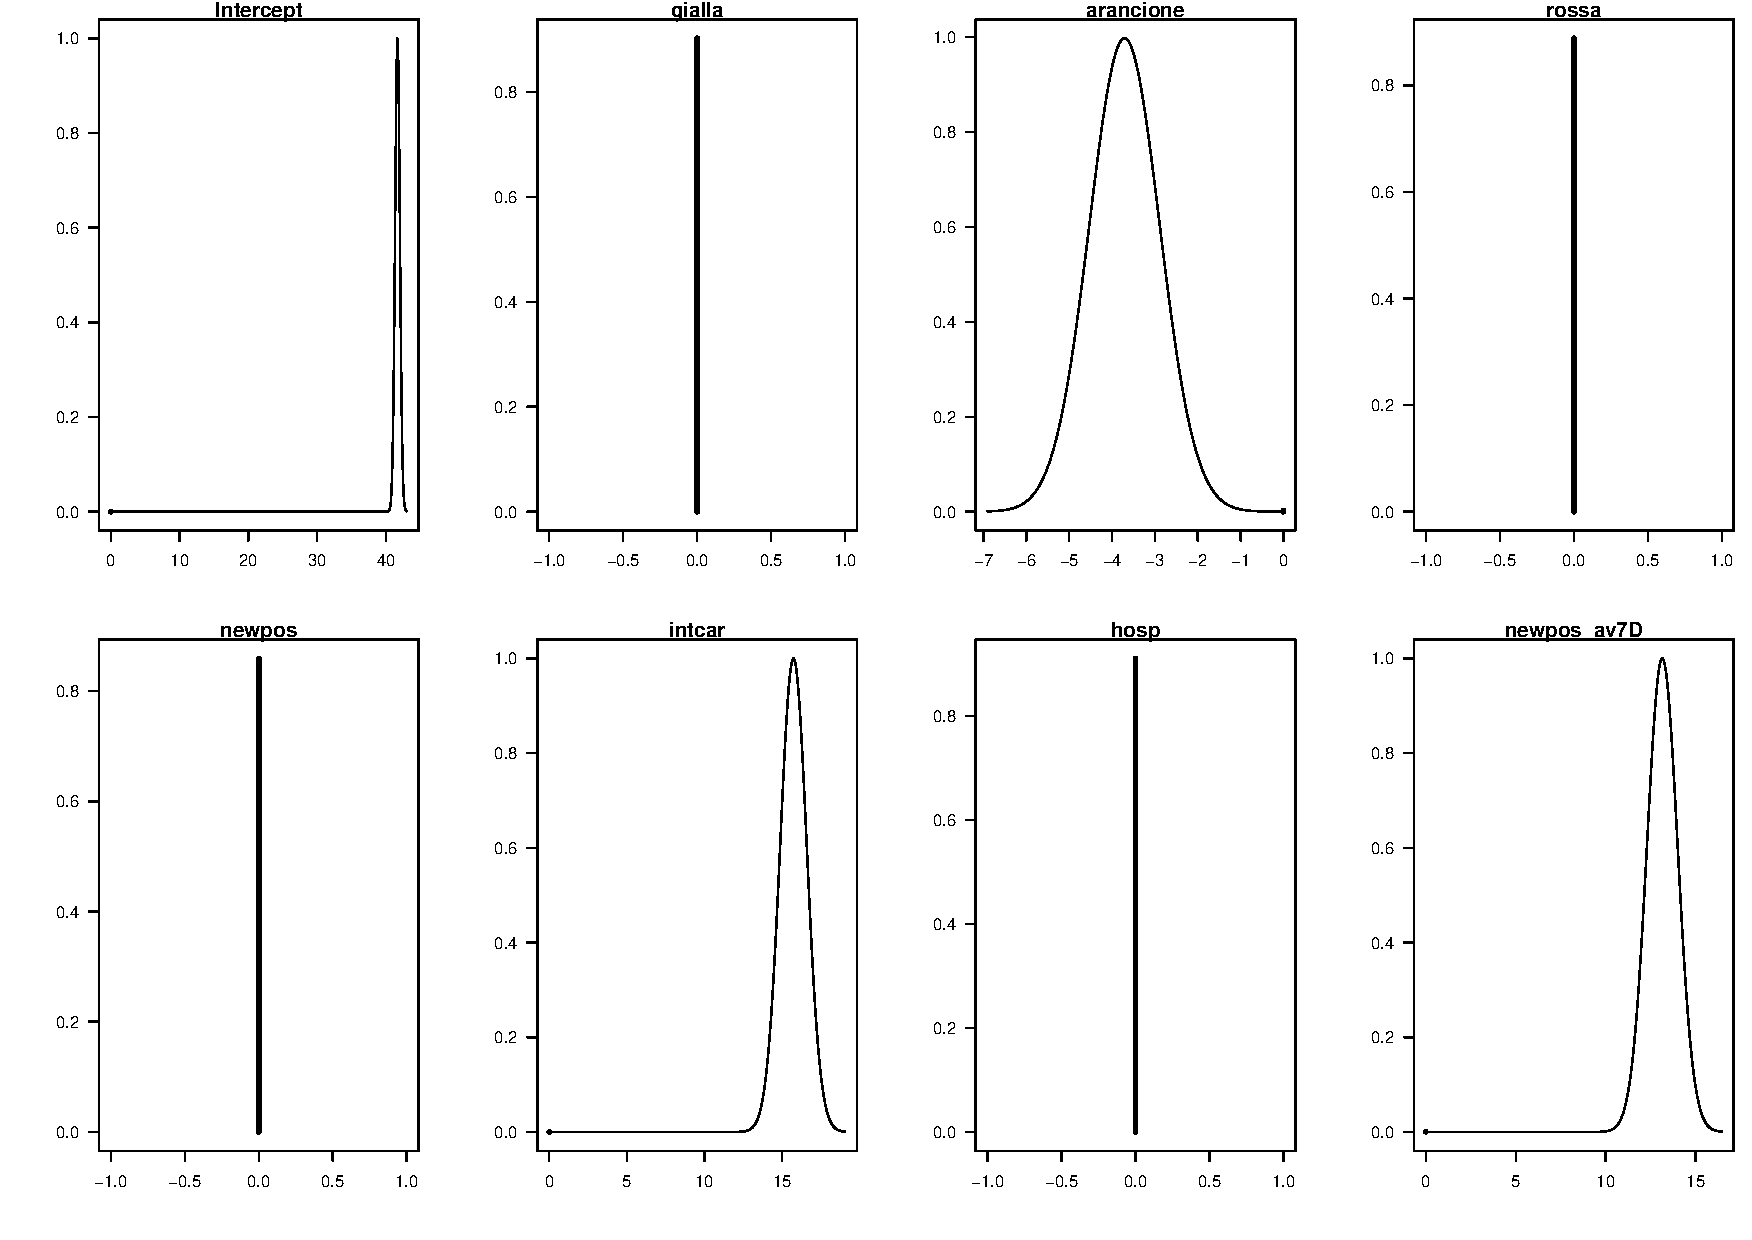
\includegraphics[width=140mm, height=90mm,scale=0.5]{posterior_2.pdf}
	\caption{Posterior distributions of coefficients for best \textbf{hospH8} model}
\end{figure}



Lastly, Table 6 shows the posterior means, standard deviations, and 95\% credible intervals.

\begin{table}[htb!]
	\centering
	\begin{tabular}{|c|c|c|c|c|}
		\hline
		Covariate         & 2.5\%  & Post. mean & 97.5\% & Post. std. dev.\\ \hline
		Intercept          & -0.03659953&-0.01249     & 0.01162539 & 0.01222                  \\ \hline
		\textbf{arancione}& -0.19703226&-0.14122  &-0.08541724   &  0.02828                       \\ \hline
		\textbf{intcar}    & 0.51756701& 0.57743   &0.63728508    &   0.03033               \\ \hline	\textbf{newpos\_av7D}     & 0.38412313 &  0.44426&0.50438846     &  0.03047              \\ \hline
	\end{tabular}
	\caption{Posterior means and standard deviations of the BMA model}
\end{table}

\newpage
\subsection{Sensitivity analysis}
Although we chose to be guided completely by the data,  we could still use a g-prior and tune the hyperparameter $\alpha$ by choosing the MSE as the criterion. We use the same models as before, so BMA with \textbf{hospH8} and the model with 3 covariates for \textbf{intcarH8}

In both cases the MSE is high for low values of $\alpha$, around 1 for both targets. However, it decreases until converges to 0.0127 for \textbf{hospH8} and 0.0495 for \textbf{intcarH8}. We settle on $\alpha = 100$. 

Since there is no substantial difference in performance we kept setting $\alpha$ to infinity, by using the \texttt{BIC} prior on BAS.

\subsection{Comparison with frequentist linear regression}
\newpage
\section{Conclusion}
\end{document}